\documentclass[crop,tikz]{standalone}% 'crop' is the default for v1.0, before it was 'preview'
%\usetikzlibrary{...}% tikz package already loaded by 'tikz' option
\usepackage[utf8]{inputenc}

\usepackage{amsmath}
\usepackage{tikz}
\usetikzlibrary{
  arrows,
automata,
backgrounds,
calc,
decorations.pathreplacing,
fit,
petri,
positioning,
shadows,
shapes,
snakes,
}

\newcommand{\tx}{\textrm{Tx}}
\newcommand{\rx}{\textrm{Rx}}
\newcommand{\listen}{\mathcal{L}}
\newcommand{\sleep}{\mathcal{S}}
\newcommand{\req}{r}
\newcommand{\ans}{a}
\newcommand{\ack}{\textrm{ACK}}
\newcommand{\racine}{root}
\newcommand{\router}{router}
\newcommand{\server}{server}
\newcommand{\act}{A}
\newcommand{\cycle}{C}
\newcommand{\txtx}{\tx \to \tx}
\newcommand{\txrx}{\tx \to \rx}
\newcommand{\rxtx}{\rx \to \tx}
\newcommand{\rxrx}{\rx \to \rx}
\newcommand{\detect}{d}
\newcommand{\pkt}{p}
\newcommand{\cmin}{c_{min}}
\newcommand{\cmax}{c_{max}}
\newcommand{\copt}{c^*}



\begin{document}

  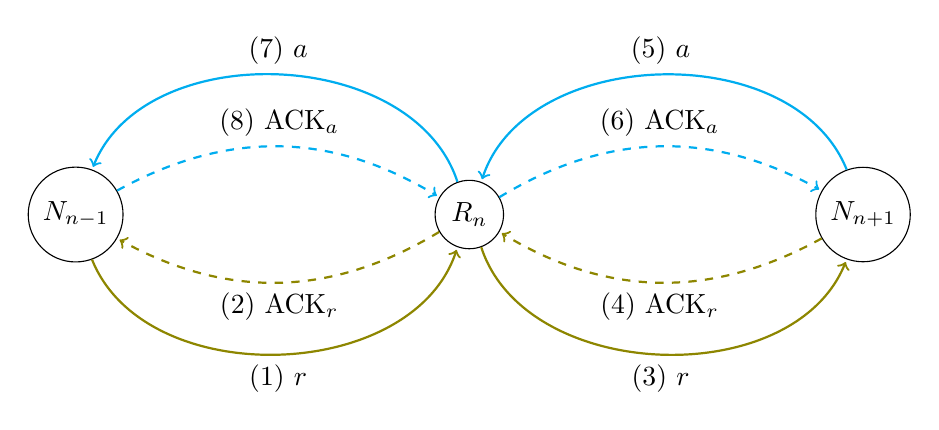
\begin{tikzpicture}[shorten >=1pt, node distance=2cm, on grid, auto]
   \node[draw, circle] (R) {$R_n$};
   \node[draw, circle] (right) [right=5cm of R] {$N_{n+1}$};
   \node[draw, circle] (left) [left=5cm of R] {$N_{n-1}$};
 
  \path[->]
    (left)  edge [bend right=70, thick, olive]   node  [below, black]   {(1) $\req$}   (R)
    (R)  edge [bend left, thick, dashed,thick, olive]   node  [below, black]   {(2) $\ack_r$}   (left)
     (R)  edge [bend right=70, thick,cyan]   node  [above, black]   {(7) $\ans$}   (left)
    (left)  edge [bend left, dashed, thick,cyan]   node  [above, black]   {(8) $\ack_a$}   (R)
    
    (R)  edge [bend right=70, thick,olive]   node  [below, black]   {(3) $\req$}   (right)
    (right)  edge [bend left, dashed, thick,olive]   node  [black]   {(4) $\ack_r$}   (R)
    (right)  edge [bend right=70, thick,cyan]   node  [above, black]   {(5) $\ans$}   (R)
    (R)  edge [bend left, dashed, thick,cyan]   node  [above, black]   {(6) $\ack_a$}   (right)
  ;
  \end{tikzpicture}

\end{document}